
%%
%% Template chap2.tex
%%

\chapter{Experiment 2: Learning with Thompson Sampling}
\label{cha:expt2}

\section{Experimental Protocol}
\label{sec:protocol2}

Studying Individual Heuristics
\begin{itemize}
	\item Split data into balanced training and test set. Use stratified shuffle split
	(similar to cross-validation) with 5 iterations
	\item Main classifier is logistic regression (one-vs-rest, L1-norm, $C=1$ for SDSS and $C=100$
	for VST ATLAS)
	\item Committee consists of 11 logistic classifiers
	\item Test 6 active learning heuristics with random sampling as benchmark
	\item Initial sample size is 50, train until we have 300 samples
	\item At each round, select a random sample of 300 and assign a score to each of them
\end{itemize}
Selection of Best Heuristic
\begin{itemize}
	\item Use Thompson Sampling to select best heuristic
	\item Still balanced split of training and test set, but now with 20 iterations of
	shuffle splits.
\end{itemize}

\section{Results and Discussion}
\label{sec:results2}
Margin appears to be the best performing heuristic in both SDSS and VST ATLAS.
To-do: add the maximum possible accuracy rate that can be achieved on plots

\subsection{Logistic Active Learning}

\begin{figure}[tbp]
	\centering
	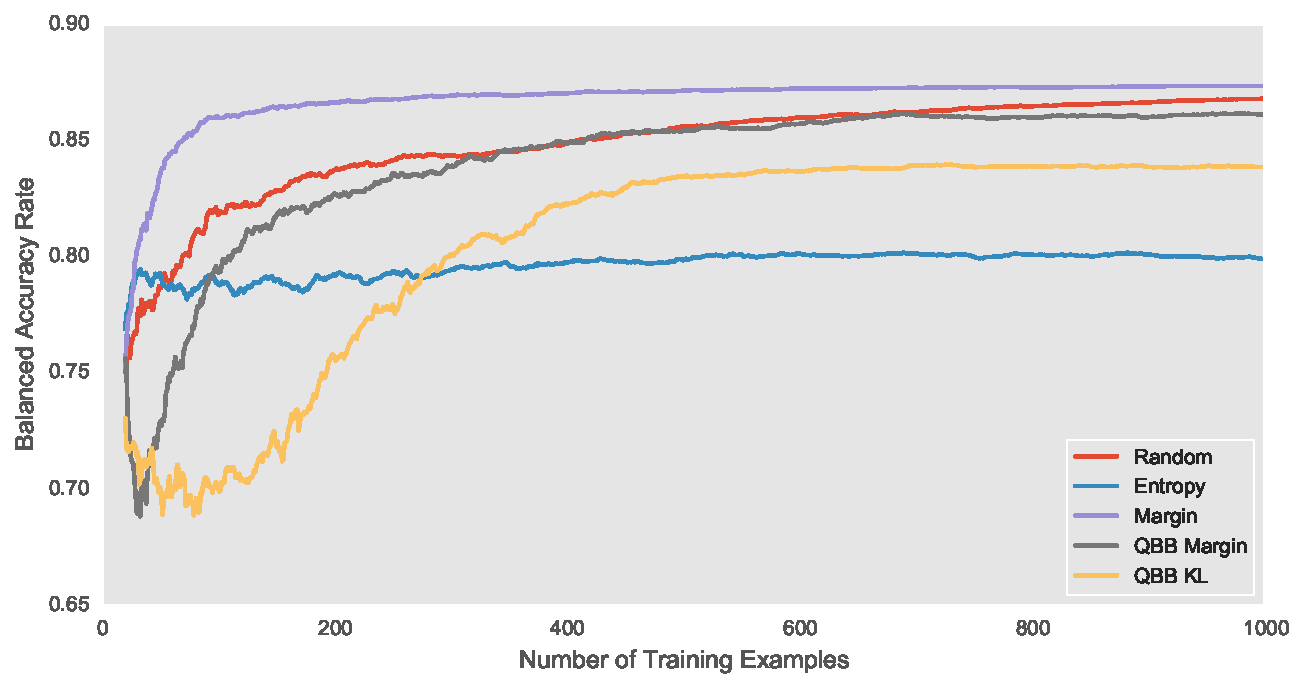
\includegraphics[width=\textwidth]{figures/lc_active_logistic_balanced}
	\caption{Learning curves of individual active learning heuristics in SDSS.}
	\label{fig:lc_active_logistic_balanced} \index{Mollweide projection}
\end{figure}

\begin{figure}[tbp]
	\centering
	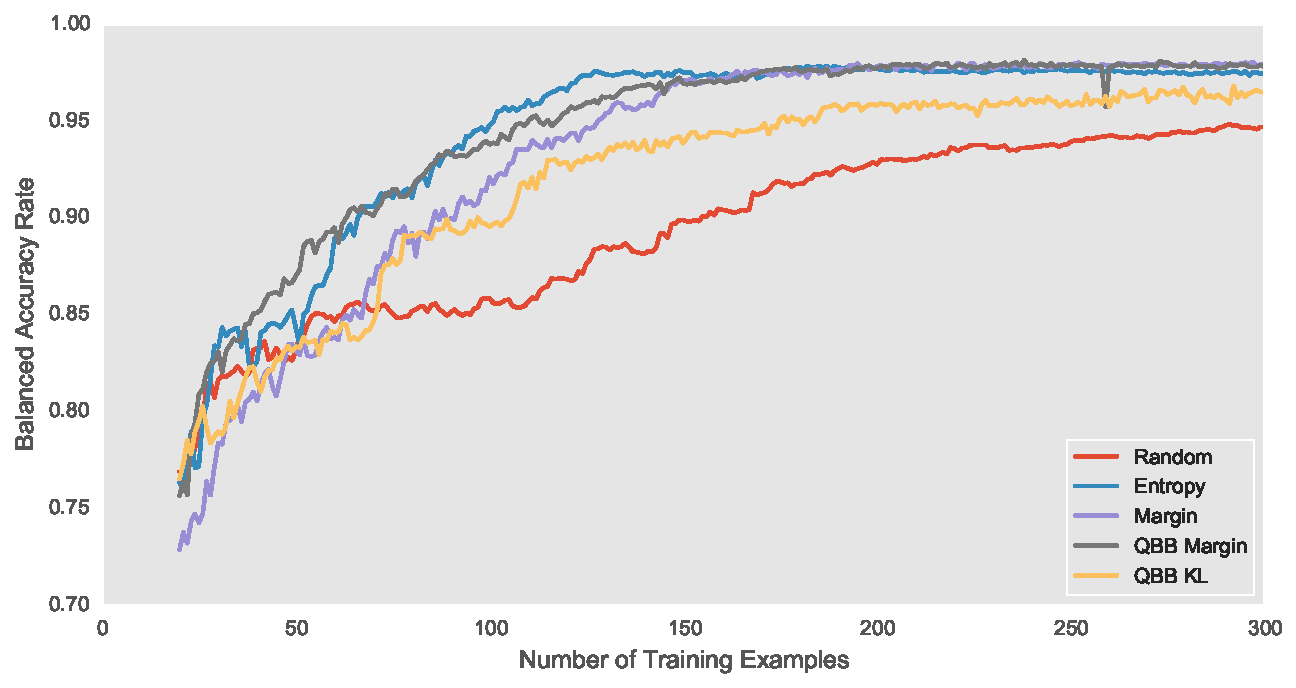
\includegraphics[width=\textwidth]{figures/active_heuristics_lc_vst}
	\caption{Learning curves of individual active learning heuristics in VST ATLAS.}
	\label{fig:active_heuristics_lc_vst} \index{Mollweide projection}
\end{figure}

\begin{figure}[tbp]
	\centering
	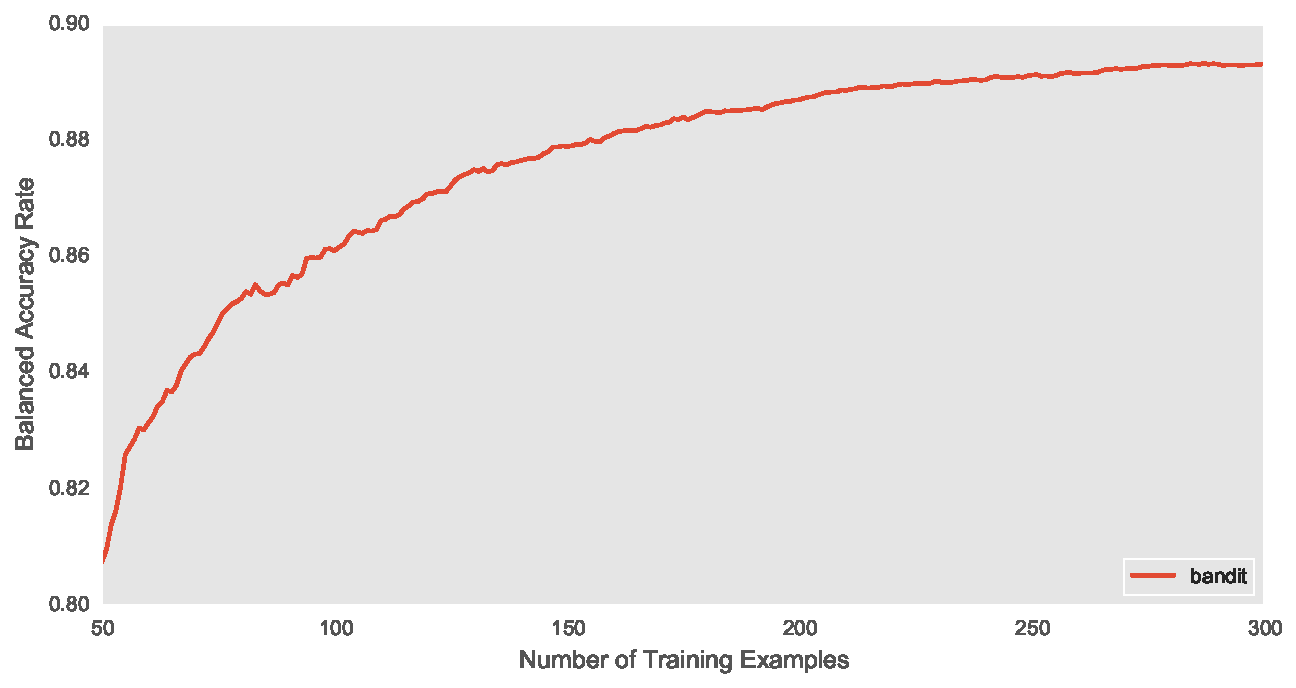
\includegraphics[width=\textwidth]{figures/bandit_lc_sdss}
	\caption{Learning curves of the bandit active learning with Thompson Sampling in SDSS.}
	\label{fig:bandit_lc_sdss} \index{Mollweide projection}
\end{figure}

\begin{figure}[tbp]
	\centering
	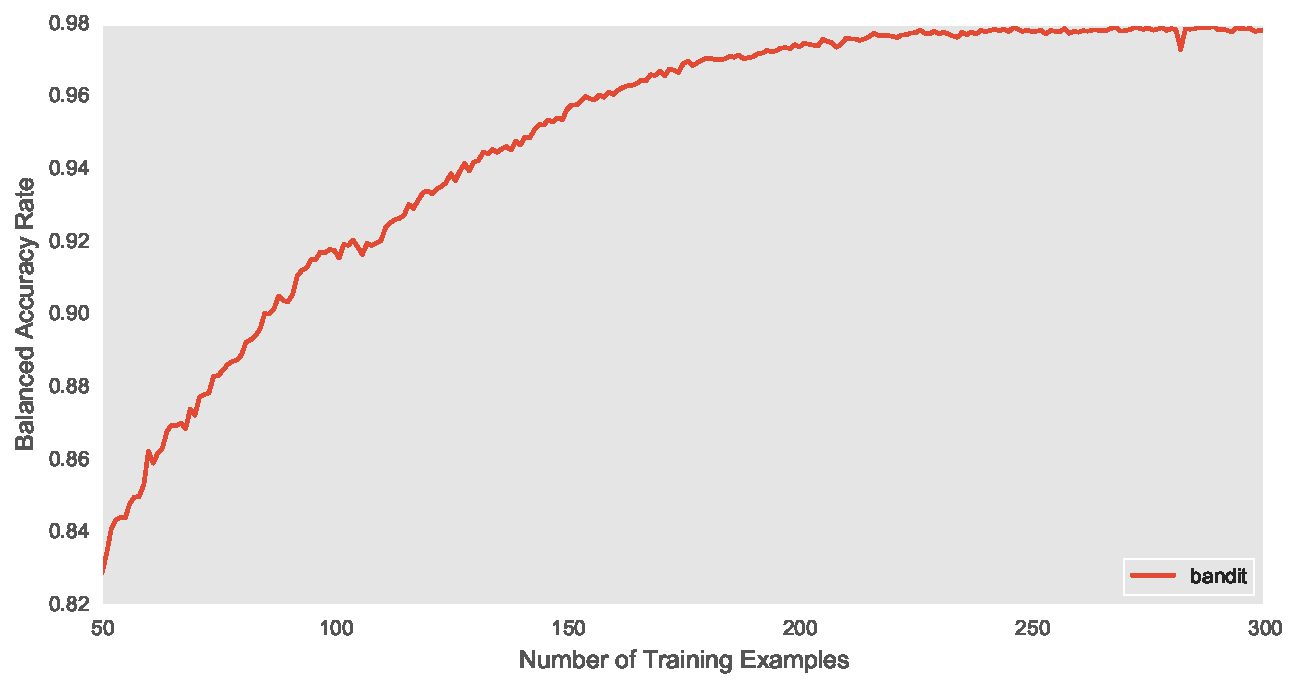
\includegraphics[width=\textwidth]{figures/bandit_lc_vst}
	\caption{Learning curves of the bandit active learning with Thompson Sampling in VST ATLAS.}
	\label{fig:bandit_lc_vst} \index{Mollweide projection}
\end{figure}

\begin{figure}[tbp]
	\centering
	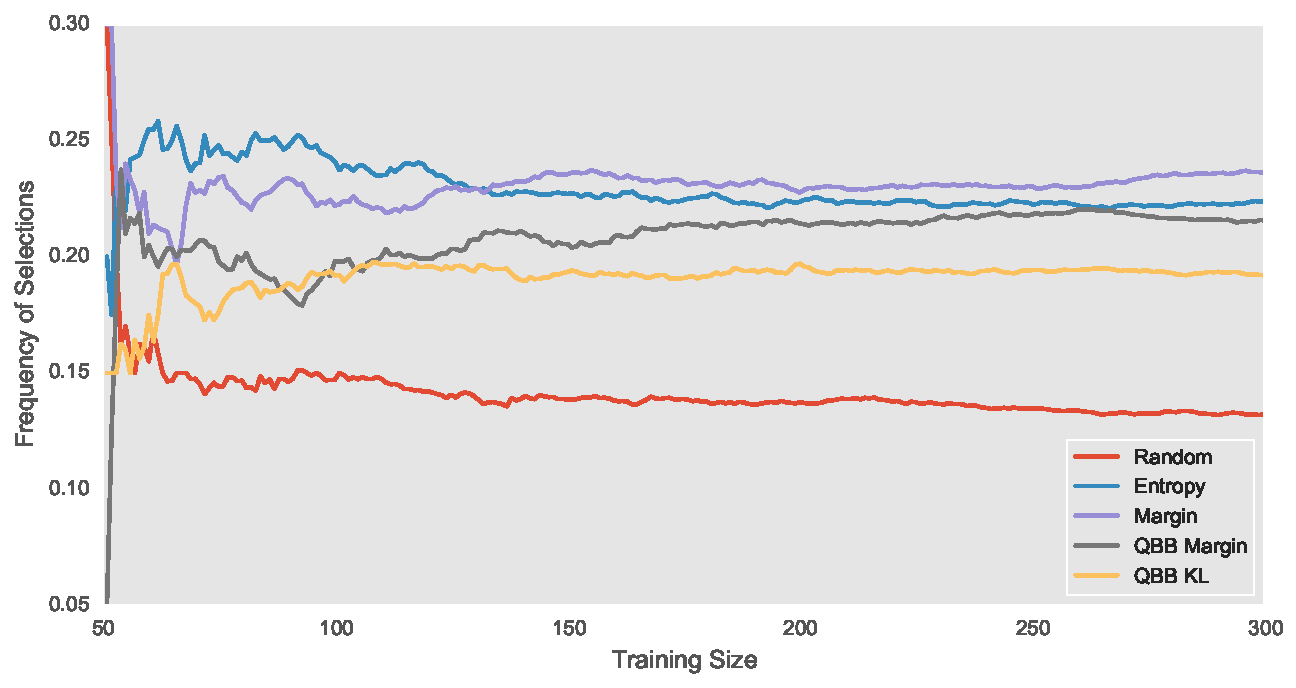
\includegraphics[width=\textwidth]{figures/bandit_sel_sdss}
	\caption{The frequency of the heuristics being selected with Thompson Sampling in SDSS.}
	\label{fig:bandit_sel_sdss} \index{Mollweide projection}
\end{figure}

\begin{figure}[tbp]
	\centering
	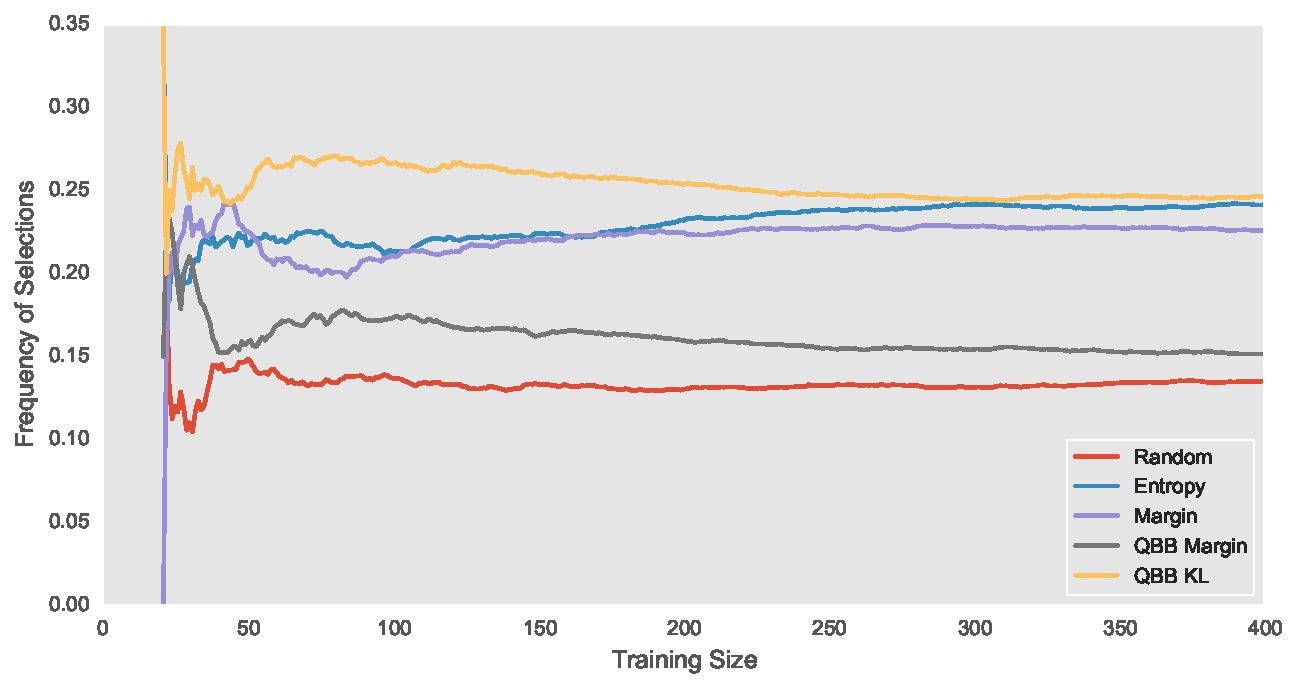
\includegraphics[width=\textwidth]{figures/bandit_sel_vst}
	\caption{The frequency of the heuristics being selected with Thompson Sampling in VST ATLAS.}
	\label{fig:bandit_sel_vst} \index{Mollweide projection}
\end{figure}


\begin{figure}[tbp]
	\centering
	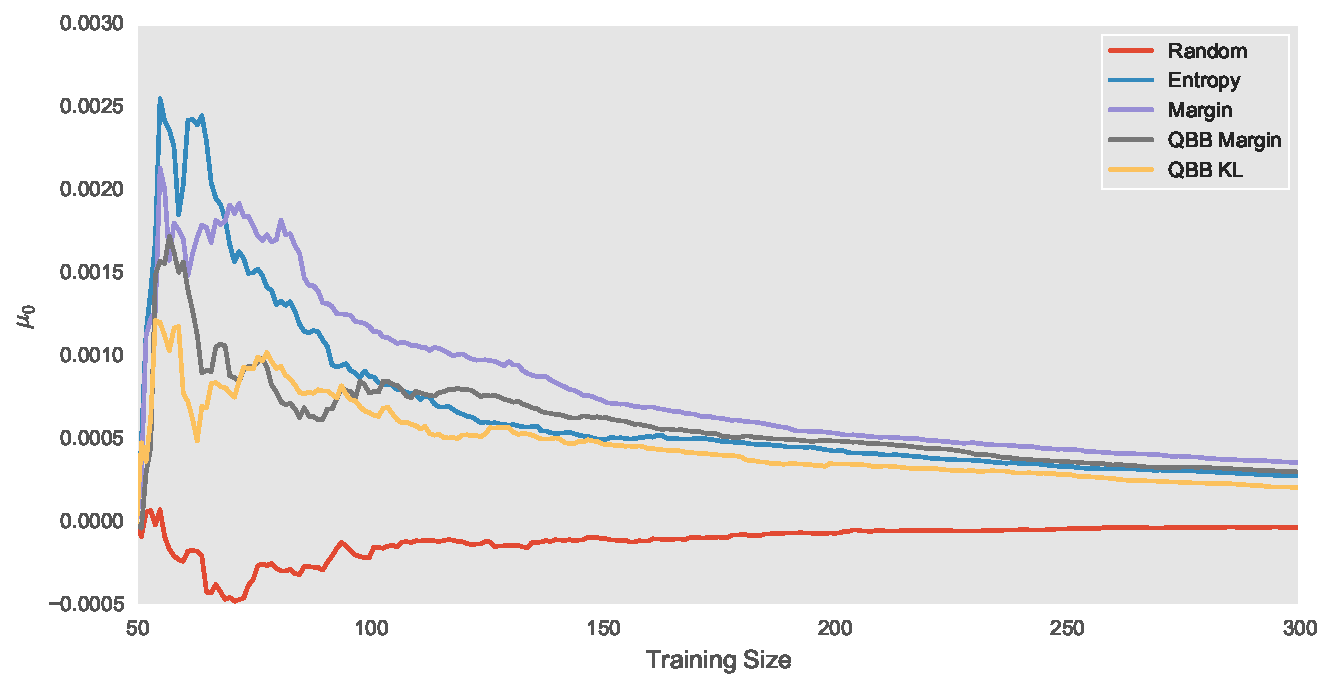
\includegraphics[width=\textwidth]{figures/bandit_mu_sdss}
	\caption{The change of the mean reward over time with Thompson Sampling in SDSS.}
	\label{fig:bandit_mu_sdss} \index{Mollweide projection}
\end{figure}

\begin{figure}[tbp]
	\centering
	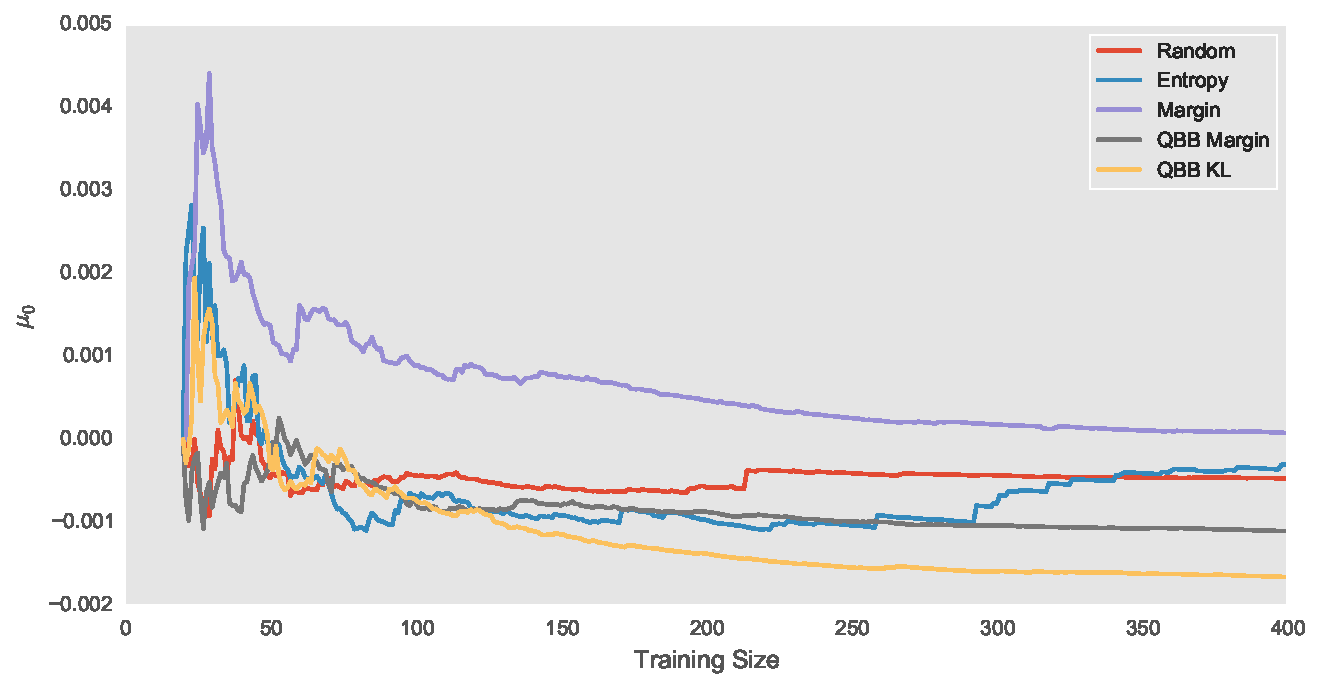
\includegraphics[width=\textwidth]{figures/bandit_mu_vst}
	\caption{The change of the mean reward over time with Thompson Sampling in VST ATLAS.}
	\label{fig:bandit_mu_vst} \index{Mollweide projection}
\end{figure}

\begin{figure}[tbp]
	\centering
	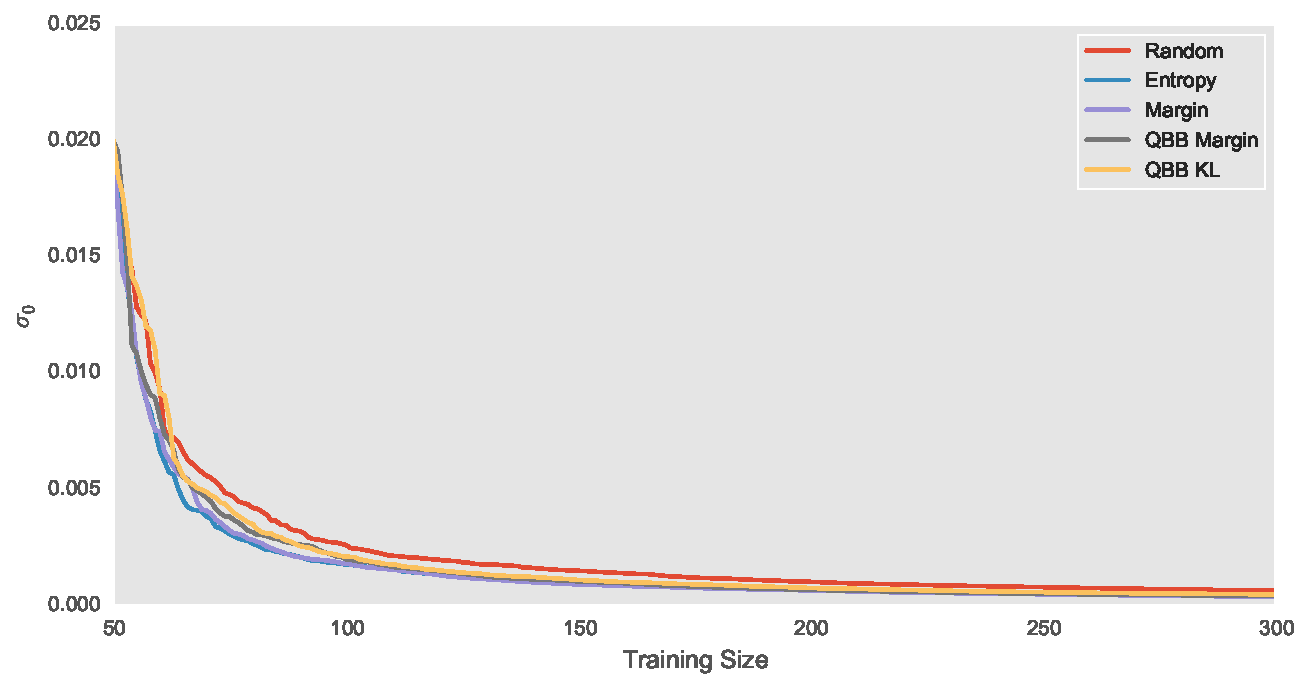
\includegraphics[width=\textwidth]{figures/bandit_sigma_sdss}
	\caption{The change in the variance of the reward over time with Thompson Sampling in SDSS.}
	\label{fig:bandit_sigma_sdss} \index{Mollweide projection}
\end{figure}

\begin{figure}[tbp]
	\centering
	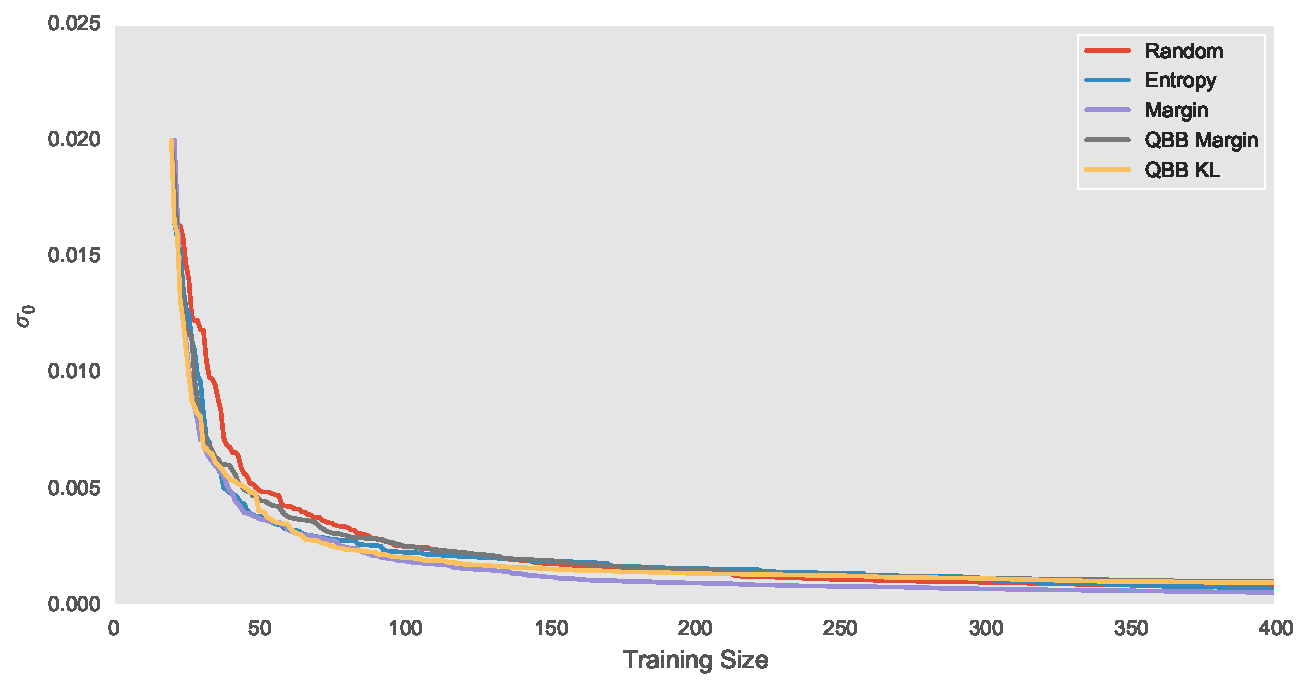
\includegraphics[width=\textwidth]{figures/bandit_sigma_vst}
	\caption{The change in the variance of the reward over time with Thompson Sampling in VST ATLAS.}
	\label{fig:bandit_sigma_vst} \index{Mollweide projection}
\end{figure}

\subsection{Heuristic Selection with Thompson Sampling}

%%% Local Variables: 
%%% mode: latex
%%% TeX-master: "thesis"
%%% End: 
